\documentclass[a4paper,12pt]{report}
    
    \usepackage[english]{babel}
    \usepackage[utf8]{inputenc}
    \usepackage{amsmath}
    \usepackage{graphicx}
    \usepackage[colorinlistoftodos]{todonotes}



    % CUSTOM MARGIN AND PARAMETER
    \usepackage[a4paper, portrait, left=1.2in,right=1in,bottom=1in,top=1in]{geometry}

    \usepackage{sectsty}
    
    \sectionfont{\fontsize{12}{1.5}\selectfont}
    \subsectionfont{\normalfont \itshape \fontsize{12}{1.5}\selectfont}
    \subsubsectionfont{\normalfont \itshape \fontsize{12}{1.5}\selectfont}
    \paragraphfont{\fontsize{12}{1.5}\selectfont}
    \chapterfont{\fontsize{14}{1.5}\selectfont}

		
    \title{Backend and Analytics as a service}
    
    \author{Aditya, Shubham, Srajan, Abhishek, Suryansh}
    
    \date{14 Oct, 2017}
    
    \begin{document}
    
    \begin{titlepage}
      \newcommand{\HRule}{\rule{\linewidth}{0.5mm}} % Defines a new command for the horizontal lines, change thickness here
      \center
      \textsc{\LARGE Shri G.S. Institute of Technology and Science}\\[1.5cm]
      \textsc{\Large Project Phase I}\\[0.5cm]
      \textsc{\large 2017-18}\\[0.5cm]
      \HRule \\[0.4cm]
      { \huge \bfseries Backend and Analytics as a Service}\\[0.4cm] % Title of your document
      \HRule \\[1.5cm]
      
\includegraphics{logo.jpg}\\[5cm] % Include a department/university logo - this will require the graphicx package    
      \begin{minipage}{0.4\textwidth}
      \begin{flushleft} \large
      \textbf{\emph{Guided By:}}\\
      Prof. D.A. Mehta
      \end{flushleft}
      \end{minipage}
      \begin{minipage}{0.4\textwidth}
      \begin{flushright} \normalsize
      \textbf{\emph{Submitted to:}} \\
      Srajan Soni (0801CS141083)\\
      Suryansh Soni (0801CS141086)\\
      Abhishek Verma (0801EC141002)\\
      Shubham Menkudle (0801CS141078)\\
      Aditya Vashishtha (0801EE141005)\\
      
      
         
      \end{flushright}
      \end{minipage}\\[2cm]            
      \vfill       
    \end{titlepage}    
    
    \begin{abstract}
    	Using an automated development tool for backend generation is a cost saving, affordable and swift approach for effortlessly creating cross platfom applications. Backend as a Service (BaaS) is the term used for providing web and mobile app developers with a way to connect their applications to backend cloud storage and processing while also providing common features such as user management, push notifications, social networking integration, and other features that mobile users demand from their apps these days. The developers can use such tools for effective backend creation and providing an integrated analytics for businesses along with these tools is the next step.
    	
    	 
    \end{abstract}
    \tableofcontents{}    
	\listoffigures

    \chapter {Introduction}    
    \section{Preamble}
    \label{sec:introduction}    
    Technology driven solutions and analytics based decision making is the core of any business in the current scenario. Moreover, creation and integration of backend and frontend for a medium sized application requires 18 weeks of time comprising of 55 percent time in backend development and average cost ranging from \$8000 to \$50,000.  Moreover in today’s scenario, there is a business urge to include statistics and other analysis to make crucial profit decisions.Growth of Analytics just as a Service is expected to be  23.4 bn dollars by 2021, and that of Backend as a service will be 208.1 bn dollars. Thenceforth, there arises the need for providing the developers with an automated tool with integrated features of backend and analytics development which will ultimately act as a profit making job in terms of cost, time and other crucial factors.
    
    \section{Need of the project}
    \label{sec:theory}
    Developing the backend and analytics services at a single platform along with the minimization of the actual coding hours is the need of the hour; thereby increasing the throughput. At the same time, due to the digitization and the demand of analytics in business sector, there is a vast opportunity for the application developers to integrate analytics solution in their applications. 
    
    But for this, the developers have to perform tedious work which usually includes a lot of redundant and unproductive jobs (including the CRUD\footnote{ CRUD - Create, Retrieve, Update and Delete operations performed on databases } applications, etc.)  eventually increasing the development time and cutting down on various other important tasks like the front end development, rigorous testing, performing critical analysis, etc. 
    
    Using automated tools for performing and maintaining CRUD operations would ease the developer's task as it will reduce the latency caused by redundant or other housekeeping jobs like authentications/authorisation, third-party logins, etc.
    
    Also, considering the analytics, the developers have to spend a lot of time studying and working on the algorithms that seems to be feasible to the situation. This also reduces the scope of algorithm comparison for the feasibility and optimality as the developer has to spend a lot of time creating different algorithms and then performing analytics with their help; so usually they come up with a theoretically optimal algorithm than a practical and tested/compared optimal ones.
    \section{Problem Statement}
    Software solution providers face constant challenge to provide a cutting edge solution to their clients along with the minimization of cost and efforts. They tackle problems related to compatibility of various technologies and constant maintenance of the software. This has been done for a long time using conventional approach of complete software coding along with a dedicated maintenance cycle. The approach has been successful but their are a lot of redundant tasks which span across projects and the goal is to minimize these tasks which can be done with minimal or no coding.    
    \section{Objectives}

    The aim of the project is - \\
    \begin{itemize}
      \item {\textbf{Stops unnecessary stack development:} Instead of many developers being forced to recreate a stack for each mobile app they develop, a BAaS service can provide for much of their underlying processing needs. The main issue would then be connecting to an API; instead of spending hours developing customized stacks, that have to be re-created, changed, and reassembled to fit the needs of each of the different app platform. Developers can build just what they need on top of the existing structures, instead of starting from scratch each time. }
  
      \item {\textbf{Allows for more accessibility: } If each app has the same underlying base, then BAaS has the potential to easily link apps across platforms. This has many benefits: from easier data sharing to better accessibility for cloud storage, a quicker spin-up time, and an overall better user experience.      }
     
      \item {\textbf{Provides diverse outcomes from one model: } Think of BAaS like a "starter home." Each user starts off with the same basic elements and continues to add over those elements to create their own customized "home." However, the base elements of the house are all the same, other users have the potential to more easily understand and even interact with or fix the "house," creating a unified backend that has a better and stronger user base. Therefore, we are reducing the redundancy of writing the same code over applications.      }
     
      \item {\textbf{Provide backend ready applications: } BAaS aims to provide the fastest way to build, deploy and manage a production application backend. To achieve this, BAaS provides a standardized architecture that  includes as much automation as possible.      }
      
      \item {\textbf{Provide a one-stop platform for various analytics: } BAaS aims at providing a platform for directly implementing the various types of machine learning and data analytics algorithms and thus enables a comparative study of algorithms on same situation and so the user(developer) could eventually choosing the most optimal as per his considerations.      }
    \end{itemize}
    \hfill
    \section{Solution Approach}
Various models are available for the development of a fully-fledged application as a developer. However taking the help of this project, the developer can have all the required functionalities and features as mentioned earlier.

As an approach to solving the problem, the developer will be provided with a software package which can be installed on the server. Various tools will be integrated and various APIs will be generated as the first step which will include the most necessary ones which are even crucial for a naive application like data APIs, auth APIs, logging and monitoring APIs and control APIs.
As a second step, various other APIs can be added by the developer which will facilitate in terms of providing fully functioning separate modules which can directly be used as end-points for their application.
The developer’s convenience to use these APIs will also be taken into consideration as in the form of providing simple and easy to use User Experience for the same.
As a parallel step, various analytical algorithms will also be developed to be provided to the developers as an on-the-go APIs/code. As a first step, we plan to integrate the most crucial 6-7 algorithms like of Classification, Clustering, Regression etc.
The user can can select from a number of algorithms available to make a fully functioning funnel \footnote{Funnel is a sequence of algorithms which operate one after another and the output of one algorithm is input to the successive one; thereby generating desired output at the end.} whose entry point will have the live data stream and output being the final/live feed or report    
\section{Organization of the Project Report}    
The report has five chapters.Chapter 1 provides introduction about the project, its need, problem statement, objectives and solution approach.Chapter 2 is focused on the background of project which includes the area, available tools, hardware and software, the references used in the projects like the research papers and their limitations.Chapter 3 includes detailed problem statement, requirement analysis, functional and nonfunctional requirements, feasibility study, and other required diagrams which better present the picture.Chapter 4 includes the architectural diagrams, with the various design issues, architecture used, along with the insights of the various models, algorithms / approaches used. Chapter 5 presents the conclusion of the report with specifying the various phase wise implementation of the project.

    
    
    \chapter {Background}        
    \section{Area}
    \subsection{Backend as a service(BaaS)}    
    Developing a mobile application from scratch is more complicated task for developers because developers couldn’t build features fast enough to keep up with market need. \\
    First you have to research and select a technology stack, write the code, connect to 1 or more 3rd party cloud APIs, test your code, deploy the stack, make it secure, and constantly version and maintain everything when you add new features or 3rd party APIs change. \\
    So the industry needed a platform to help developers manage the complex balance between need and supply. This need gave birth to BaaS. \\    
    Backend as a service (BaaS) is a cloud computing architecture that provides mobile applications with access to servers, storage, databases and other resources that they need to run on – quickly and effortlessly. BaaS is disrupting the traditional ‘Mobile Enterprise Application Platform’ for today’s businesses by offering more turn-key functionalities than conventional API management to create better user experience (UX). \\
    
    \subsection{Analytics as a Service}    
    For years, IT organizations have generated, collected and stored vast amounts of data. Now, IT is being asked not just to store the data but to provide the infrastructure to perform analytics on it. The trouble is that the task is a resource-intensive proposition. \\    
    According to Alex Barret[8],Analytics as a service (AaaS) refers to the provision of analytics software and operations through web-delivered technologies. These types of solutions offer businesses an alternative to developing internal hardware setups just to perform business analytics. \\
    \subsection{Available Tools}
    Some of the popular BaaS tools available are :
    \begin{itemize}
    \item Firebase
    \item Parse
    \item Kinvey
    \item Cloudboost
    \end{itemize}
    
    \subsection{Hardware tools}    
    \begin{itemize}
    \item A dedicated server with minimum 1GB of RAM
    \end{itemize}

    \subsection{Software tools}    
    \begin{itemize}
    \item NodeJS     
    \item Python
    \item MongoDB
    \end{itemize}
            
    \section{Literature review}
    BaaS has been a recent trend in the application development industry.It aims to boost up the development process,thereby saving time and cost.The literature review will focus on the keywords of the problem,its pros and cons.The review is majorly based on work done by Phy Nguyen[7].
    
    \subsection{Backend as a Service (BaaS)}
    In this section,pros and cons of BaaS will be discussed. \\
    \subsubsection{Pros :}
    \begin{itemize}
      \item More focus on UI/UX.
      \item More extensible with less efforts.
      \item Cross platform apps with one common backend.
      \item Development and Analytics at one place.
      \item Easy visualisation and Real time analysis      
      \item Customisable analytics options      
      \end{itemize}
      \subsubsection{Cons :} 
      When it comes to disadvantages of a service, these are the categories :  control, scalability, and shutting-down probability. 
      \begin{itemize}
        \item Firstly, when an organisation has an application running over a BaaS, there is no complete control over its infrastructure and software stack (APIs, SDKs). 
        \item Secondly, features of BaaS are not suitable for large-scale applications. 
        \item Lastly, the risk that an organisation takes when they use BaaS, is that the service might get taken down and they will face a severe amount of data migration to a new backend system.
      \end{itemize}   
    
    \subsection{Analytics as a service}
    \subsubsection{Pros}
    \begin{itemize}
      \item Allows users to focus on exploring and analyzing data      
      \item Teams can spend their time exploring the data, formulating hypotheses and discussing insights with collaborators.      
    \end{itemize}
    
    \subsubsection{Cons}
    \begin{itemize}
      \item Might be a risky step.
      \item Cost and time required to transfer data to the AaaS provider.      
    \end{itemize}

    \chapter {Analysis}
    \section{Detailed Problem statement}
    \label{sec:theory}
    Backend is considered to be backbone of any application regardless the platform it is made for, since it is the backend which deals with basic CRUD operations involved in an application and it also provide data persistency. But still the major focus from users perspective is on front end or user interface,but developers on standard, put only 40% of their effort for front-end part remaining in backend related task. \\
    The amount of work involved in creating this backend technology is never a simple task, there is a demand for various types of applications which demand to be completed within the prescribed deadlines. \\
    It takes almost 18 weeks to develop and publish a standard native mobile application, which include almost 10 weeks to built a back-end and around 8 weeks to build the front-end.\\
    The backend task contains a set of hectic steps in traditional approach including the following steps-\\
    Envisioning - 2-4 weeks.\\
    Iterative Development and Testing - 6-8 weeks.\\
    Stabilization - 1-2 weeks.\\
    Release - 2 weeks.\\
    So, Total time (traditional approach) \\
    App Making Cost = (UI/UX Design Hours + iOS App Hours + Android App Hours + Backend Server Hours) X Developer’s Hourly Rate.\\    
    Moreover, in today’s scenarios as growing data and digitalisation of systems, the data can be used in various analytics related application, which has even worse condition since even small analytics requires a lot of effort to build on to the top of already developed application.\\    
    Mobile computing is growing rapidly many applications are cross-platform, and to create cross platform application we need centralised database which will support CRUD for various platform.\\
    Hence to provide Backend and Analytics as a service, which deals with to provide API based automated solution to backend and analytics in a single unit. It will target to automate simple backend and analytic related task and provide endpoint APIs for the same.\\    
    \section{Requirement Analysis}    
    \subsection{Functional Requirement}
    \begin{enumerate}
      \item {\emph {Create schema :} User will be provided with option to create a schema of database to have initial database structure. \\
      Input- Schema design as per the user’s (developer’s) need.  \\
      Output- Database table structure with all the required dependencies as per the schema.}
      \item {\emph {Create Template :} Based on the schema now user can choose the template (json structure as query response) as to retrieved when he hit the API. \\
        Input- Template format, chosen structure. \\
        Output- Data will be provided in the chosen format.
      }
      \item {\emph {Generate Endpoint :} Based on the schema now user can choose the template (json structure as query response) as to retrieved when he hit the API. After creating his template user can generate endpoint either in public or user specific mode.\\
        Input- Choose to create endpoints and mode. \\
        Output- Display the successful endpoints in an organised and easy to access way.
      }
      \item {\emph {Customize Template : } User is provided with option to customize template as per his need hence further modification for same endpoint.\\
        Input- Choose an endpoint and make customizations (Input as a new customised template).\\
        Output- Updated the modified template to the user’s area.
        }                        
      \item {\emph {Authenticate Endpoint :}If user has selected for private access as per some id or database schema column, he can authenticate that endpoint.\\
        Input- Choose private access for the desired schema and provide some security code (id).\\
        Output- Authenticated schema (accessible only by valid authority).
      }
      \item {\emph {Generate Key : }For authentication purpose a private and public key combination is generated.\\
        Input- Get user’s credentials. \\      
        Output- Generate unique authentication id and update/store it to database.
      }
      \item {\emph {Match Key :} If user has selected for private access as per some id or database schema column, he can authenticate that endpoint.\\
        Input- Request API access with unique Id. \\
        Output- Provided authorization to that API.
      }
      \item {\emph {Use Custom Queries : }  User will be provided with flexibility to write his own queries in case if he need more hold on the retrieved results. \\
        Input- Updated query with selected API and user’s Id. \\
        Output- Query updated for particular user area and results modified.      
      }
      \item {\emph {Show stats :} Stats such as number of active user, total API hits etc will be shown on the dashboard. \\
        Input- Visit Dashboard update (auto refresh). \\
        Output- Current status of active users, API hits, etc.
      }
      \item {\emph {CRUD Operation :}  Operations such as Create, read, update and delete in background if user hit the API endpoint. \\
        Input- API endpoint, with user id; data, and action to work on. \\
        Output- Update the database and notify the user.
      }
      \item {\emph {Logging Info :} Informations related to exception, Access etc are logged for future references. \\
        Input- Real time website data. \\
        Output- Logging details i.e. based on IP, page clicks, exception or error etc.  
      }
      \item {\emph {Export Data : } Export data stored in schema or other logs related to statistics can be dump into various formats. \\
        Input- Select schema or info to export and file format.\\
        Output- Export data in standard file format eg csv, xml, json etc.  
      }
      \item {\emph {Import Data :}  Options Available to import the data from some predefined file format. \\
        Input- Select import file and its file format. \\
        Output- Data imported according to file format in schema.
      }
      \item {\emph {Create Funnel :}   For analytics creating funnel that is json structure to algorithm for analysis on the data (constrained to data type supported by algorithm) \\
        Input- Schema and algorithm. \\
        Output- Endpoint which give result of analytics algorithm in chosen schema.  
      }
      \item { \emph {Choose Labels :} Select features from specific schema to apply algorithm/funnel. }
      \item {\emph {Generate Graphs :}   Generate graph on the basis of insights generated from the analysis. \\
        Input- Select attributes from the set of all relevant attributes, for plotting the graph.\\
        Output- Generated graph corresponding to the data on specified attributes.
      }
      \item {\emph {Generate Summary :}    Small summary based on the analytics results. \\
      Input- Select the data-set to be summarised.\\
      Output- Brief summary related to the trends or any anomaly, etc.
      }
      \item {\emph {Aggregation functions :} Availability of default aggregation function such as Min, Max, Mean, Mode etc for direct usage. \\
        Input- Calls to the predefined (custom-made) functions, and parameters to work upon. \\
        Output- Output the results related to the desired function.
      }
      \item {\emph {Social Media Login/Logout :} Social media integration such as login via facebook, google+, twitter etc. \\
        Input- Choosing the third-party, application ID and secret key. \\
        Output- Third-party login service will be embedded.
      }
      \item {\emph {File storage : } API endpoints specifically for data files in case if files are stored. \\
        Input- Choose for file handling operations. \\
        Output- Output or make the desired changes.
      }
      \end{enumerate}
    \subsection{Non-Functional Requirement}
    \begin{enumerate}
      \item {\emph {Security :} 
      The security in every aspect will be taken into consideration by various authentication and authorization processes at every crucial place like API access, data entry, customization, etc.      
      }
      \item {\emph {Reliability :} 
      The APIs will be created as a full and tested ready-to-use code which will ensure a reliable services.
      }
      \item {\emph {Flexibility :} 
      Change and modification in functionalities is easier. For a large scale application, modification in features without affecting other functionalities is desired.
      }
      \item {\emph {Reusability :} 
      Provides a vast reusable code in the form of APIs, algorithms, etc. Also the customization in the APIs could also be used further so the customized query and other factors.
      }
      \item {\emph {Maintainability :} 
      The control over the application is an aid as the modules can be easily tested for bugs or enhancements which are usually loosely coupled. So a module wise implementation ensures individual maintainability as well.
      }
      \item {\emph {Extensibility :} 
      Adding new features and functionalities to an existing system becomes easier and faster with already available APIs. 
      }
      \item {\emph {Auditability :} 
      With the logging and monitoring tools, any anomaly and inoperable state are communicated in real time.      
      }
    \end{enumerate}
    \section{Feasibility Study}    
    \begin{enumerate}
      \item {\textbf{Economical :} 
      Languages tools and software which are used to develop the product are easily available for free.
      }
      \item {\textbf{Technical :} 
      Tools and software needed for realisation of the system such as NodeJS, Python, C etc are easily available and can be integrated.
      }
      \item {\textbf{Operational :} 
      Proposed system will be operationally very efficient it will guarantee to reduce total application development time by at least 30%+ which is a very great amount of time 
      }
    \end{enumerate}

    \chapter {Design}
    \section{Preface}
    The diagrams that are necessary to analyse, visualize and evaluate the system are discussed in this chapter. Architecture, use case and ER diagrams are created to know the complete design of the system.
    \section{Diagrams}          
      
      \begin{figure}[h]
        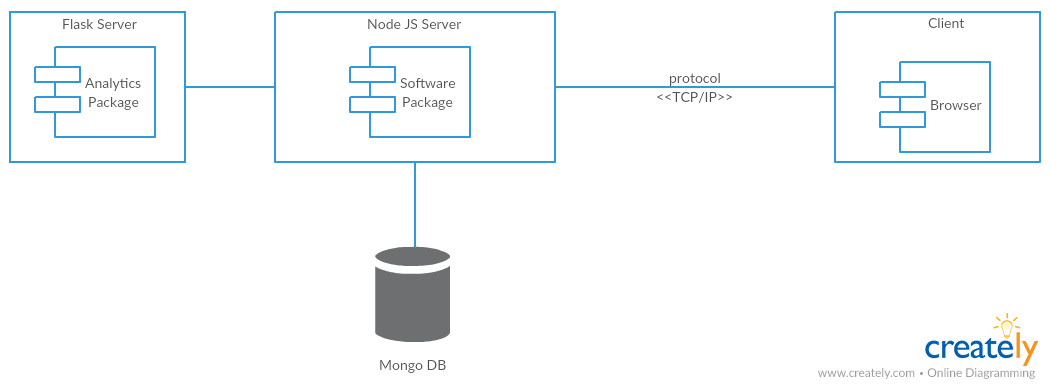
\includegraphics[width=1\textwidth]{Deployment.png}
        \caption{ Deployment Diagram}  
      \end{figure}
    
    \newpage          
    \begin{figure}[h]
      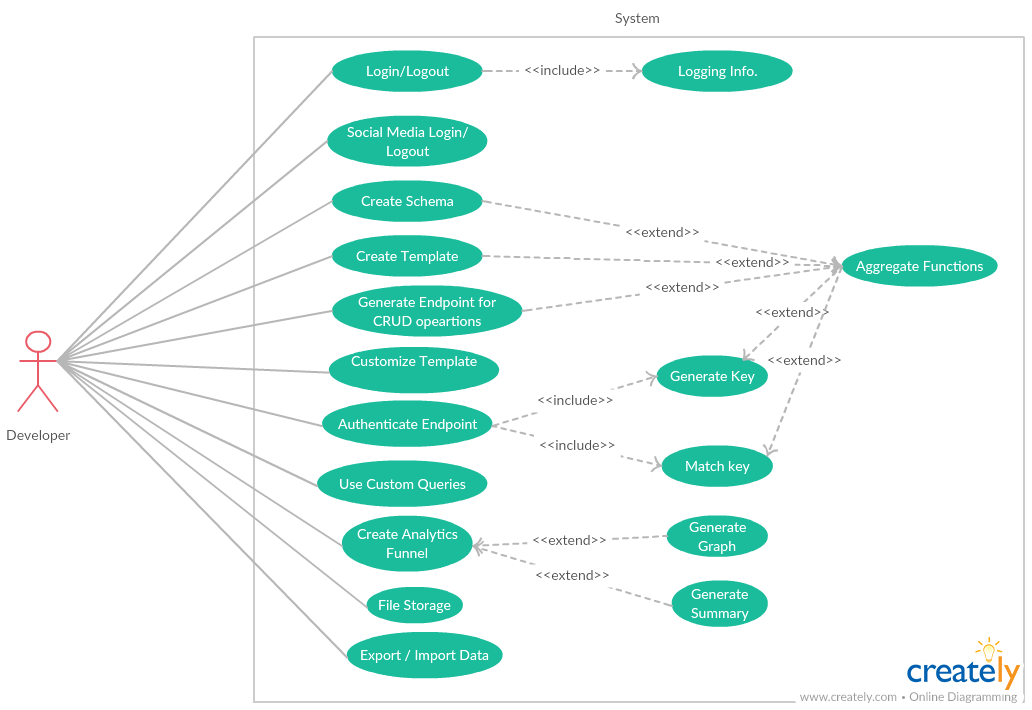
\includegraphics[width=1\textwidth]{usecase.png}
      \caption{ Usecase Diagram}  
    \end{figure}
	\newpage
	\begin{figure}[h]
      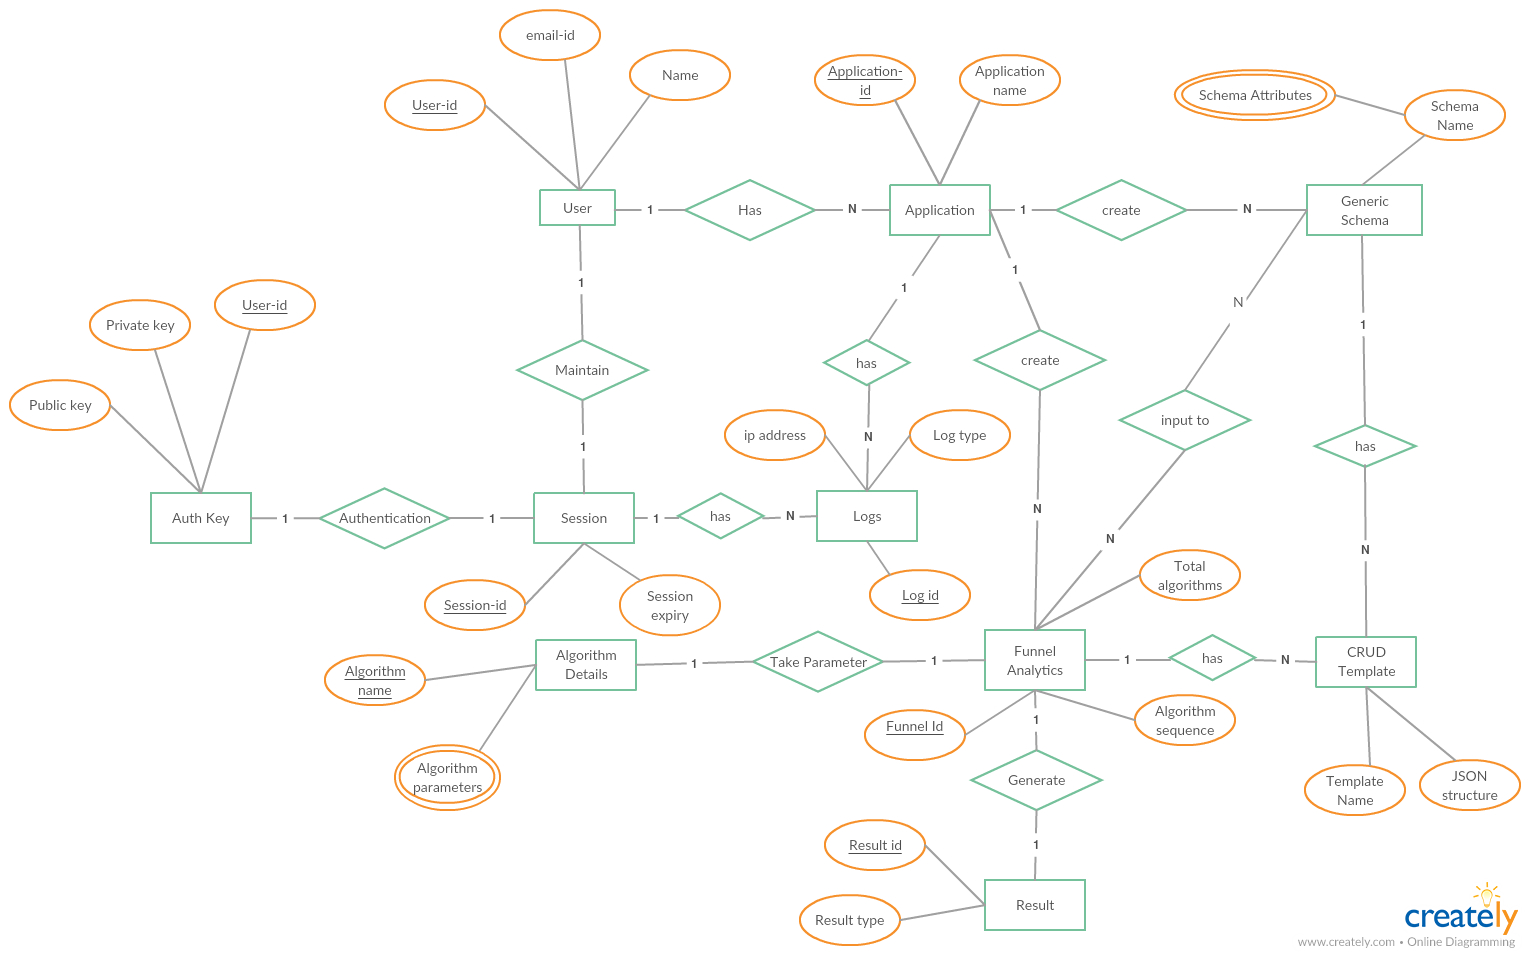
\includegraphics[width=8.5in ,angle=90]{ER.jpg}
      \caption{ ER Diagram}  
    \end{figure}

    \chapter {Conclusion}
    \section{Work carried out in phase 1}
    \begin{itemize}
      \item  Detailed study of Existing Systems
      \item  SRS(Software Requirement Specification)
      \item  Project Report and documentation
      \item  Finalised functional and nonfunctional requirements and features
      \item  Finalised our technology stack
    \end{itemize}
    \section{Work to be carried out in phase 2}
    \begin{itemize}
      \item  Creating User Interface and Configuring server
      \item  Implementation of the software package
      \item  Creating Endpoints for the algorithms
      \item  Implementation of analytical tools 
    \end{itemize}    
    
    \renewcommand{\bibname}{References}
    \begin{thebibliography}{9}
    \bibitem{nano3}
    	Francis Gropengießer and Kai-Uwe Sattler,
      \emph{Database Backend as a Service: Automatic Generation, Deployment, and Management of Database Backends for Mobile Applications}.
			Available at https://link.springer.com/article/10.1007/s13222-014-0157-y
			
		\bibitem{nano3}
      \emph{Overview Of Backend as a Service (BaaS) White Paper}.
			Available at http://baas.apievangelist.com/2013/05/08/overview-of-backend-as-a-service-baas-white-paper/
			
								
		\bibitem{nano3}
			Balkan, A. 2012,
      \emph{What are the pros and cons of using a backend as a service?}.
			Available at https://www.quora.com/What-are-the-pros-and-cons-of-using-a-backend-as-a-service
		
		\bibitem{nano3}
			Backend as a Service (BaaS) Market Global forecast for 2020,
			Available at http://www.marketsandmarkets.com/PressReleases/baas.asp		
		
		\bibitem{nano3}
			Backendless website 2016,
      \emph{Database Backend as a Service: Automatic Generation, Deployment, and Management of Database Backends for Mobile Applications}.
			Available at https://backendless.com/what-is-backend-as-a-service/
	

		\bibitem{nano3}
			Ryan Goodrich,
      \emph{What is BaaS (Backend as a Service)}.
			Available at http://www.businessnewsdaily.com/4992-what-is-baas.html	
			
		\bibitem{nano3}
			Nguyen, T, 2016,
      \emph{Mobile Backend as a Service: The Pros and Cons of Parse
			Case company: SuperApp Oy}.
			Available at http://theseus.fi/bitstream/handle/10024/117483/Nguyen{\_}Phu.pdf?sequence=2
		
		\end{thebibliography}	
    \end{document}\grid
